\subsection{Transfer to bearings, ECG, and synthetic cycles}
\label{sec:transfer-main}

\paragraph{Setup reminder.}
Table~\ref{tab:transfer-main} reports the primary metric \textbf{locked $R_{\mathrm{blend}}$} (higher better; $\alpha{=}0.7$ seam/body blend from Section~\ref{sec:residual-score}) after training/searching DenoiseOpt
(\texttt{hybrid\_lstm}, seed \texttt{1902771841}) on each transfer board
from Section~\ref{sec:transfer-protocol} ($n{=}256$ periods, $L{=}256$).
No PESQ/STOI/MOS appears on these boards: periods are non-speech wrap tiles, and the claim is wrap-protocol residual repair only.
Columns are: CWRU/MFPT/Paderborn bearing revolutions, MIT-BIH/PTB-XL ECG beats, and synthetic CNC/PMU pilots.
Numbers come from the released
\href{https://github.com/reeldemo/reelsynth/blob/main/brand/artifacts/signal_heal_transfer/results_table.json}{results\_table.json}
(\texttt{primary\_metric=r\_blend}).
Domain-trained Noise2Noise-style SeamN2N (corrupt$\to$corrupt, $4000$ Adam steps, train seed \texttt{424242}, holdout seed \texttt{20260719})
is scored on the same seven boards under the \emph{same} $R_{\mathrm{blend}}$.
Author ECG Cycle-GAN and BeatDiff remain OOD wrap probes on ECG only
(clinical restore $\neq$ wrap residual, Table~\ref{tab:transfer-sota-status}).
These rows do \emph{not} transfer an audio-trained bake as fault/ECG diagnosis SOTA; they only stress the wrap geometry.
Artifacts:
\href{https://github.com/reeldemo/reelsynth/tree/main/brand/artifacts/signal_heal_transfer}{signal\_heal\_transfer}.

\begin{table}[t]
  \centering
  \caption{Wrap-heal transfer under locked $R_{\mathrm{blend}}$ (higher better; wrap-protocol stress test).
  Bearing boards ($n{=}256$ each). DenoiseOpt: \texttt{hybrid\_lstm}, seed \texttt{1902771841}.}
  \label{tab:transfer-main}
  \setlength{\tabcolsep}{3pt}
  \footnotesize
  \begin{tabular}{@{}lccc@{}}
    \toprule
    Method & CWRU & MFPT & Paderborn \\
    \midrule
    Ours & 0.960 & 0.943 & 0.937 \\
    SeamN2N & 0.866 & 0.866 & 0.842 \\
    no-bake & 0.845 & 0.866 & 0.838 \\
    endpoint-pin & 0.505 & 0.545 & 0.567 \\
    \texttt{seam\_fir3} & 0.448 & 0.573 & 0.560 \\
    DualCosine & 0.461 & 0.483 & 0.471 \\
    \bottomrule
  \end{tabular}
\end{table}

\begin{table}[t]
  \centering
  \caption{Wrap-heal transfer under locked $R_{\mathrm{blend}}$ (continued): ECG and synthetic boards.
  BeatDiff / Cycle-GAN are author OOD wrap probes on ECG only.}
  \label{tab:transfer-main-b}
  \setlength{\tabcolsep}{2.5pt}
  \footnotesize
  \begin{tabular}{@{}lcccc@{}}
    \toprule
    Method & MIT-BIH & PTB-XL & CNC & PMU \\
    \midrule
    Ours & 0.975 & 0.945 & 0.991 & 0.992 \\
    SeamN2N & 0.750 & 0.754 & 0.553 & 0.959 \\
    no-bake & 0.750 & 0.762 & 0.450 & 0.936 \\
    endpoint-pin & 0.865 & 0.870 & 0.410 & 0.944 \\
    \texttt{seam\_fir3} & 0.766 & 0.760 & 0.534 & 0.912 \\
    DualCosine & 0.414 & 0.512 & 0.494 & 0.827 \\
    BeatDiff (OOD) & 0.491 & 0.493 & --- & --- \\
    Cycle-GAN (OOD) & 0.106 & 0.211 & --- & --- \\
    \bottomrule
  \end{tabular}
\end{table}



\begin{figure}[t]
  \centering
  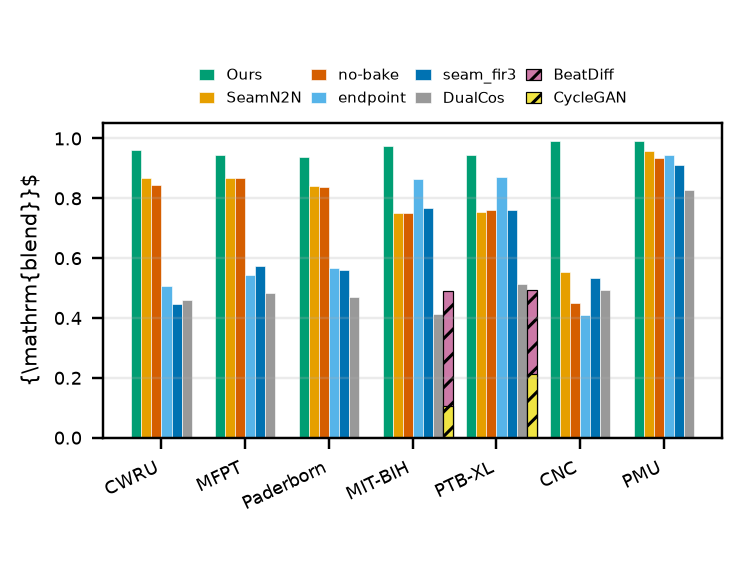
\includegraphics[width=\columnwidth]{figures/fig_signal_heal_transfer.png}
  \caption{Grouped bars for Tables~\ref{tab:transfer-main}--\ref{tab:transfer-main-b}: $R_{\mathrm{blend}}$ by board and method
    (higher better). Core rows (Ours, SeamN2N, no-bake, endpoint-pin, \texttt{seam\_fir3}, DualCosine)
    appear on all seven boards. Hatched bars are author OOD wrap probes on ECG (BeatDiff, Cycle-GAN)
    and the Paderborn Al~Firdausi architecture-reuse wrap bake
    (not the published fault classifier, see Table~\ref{tab:transfer-sota-status}).
    Missing cells are omitted rather than zero-filled.}
  \label{fig:signal-heal-transfer-main}
\end{figure}

\begin{table}[htbp]
  \centering
  \caption{Author-method and data-cut status under this wrap-protocol stress test (no invented scores).}
  \label{tab:transfer-sota-status}
  \setlength{\tabcolsep}{3pt}
  \resizebox{\columnwidth}{!}{%
  \begin{adjustbox}{max width=\columnwidth}
\begin{tabular}{@{}lp{0.52\columnwidth}@{}}
    \toprule
    Scope & Note \\
    \midrule
    SeamN2N (ours, N2N-style) & Scored on all seven Table~\ref{tab:transfer-main} boards
      under $R_{\mathrm{blend}}$. Not Lehtinen code \\
    Cycle-GAN (ECG, author) & OOD wrap probe in Table~\ref{tab:transfer-main}
      (MIT-BIH $0.1063$, PTB-XL $0.2105$). Clinical restore $\neq$ wrap residual \\
    BeatDiff (Bedin NeurIPS\,2024) & OOD wrap probe in Table~\ref{tab:transfer-main}
      (MIT-BIH $0.4907$, PTB-XL $0.4933$). Drive prior (not HF).
      Clinical morph prior $\neq$ wrap residual \\
    Paderborn KAt deep (Al~Firdausi CNN) & Trained CNN\_1D\_2L from scratch (not frozen
      \texttt{model.pth}) on bearings K001/KA04/KI04/KB23. File-holdout seed \texttt{20260726},
      train seed \texttt{42}, $20$ epochs. 4-class holdout acc $0.8590$ ($n{=}2560$ segs,
      NORMAL/IR/OR/OR+IR). Classifier wrap residual N/A. Arch-reuse wrap bake listed
      in Table~\ref{tab:transfer-main}$^\dagger$.
      Wrap board: Ours $0.9369$ / SeamN2N $0.8421$ / DualCosine $0.4710$ \\
    Expanded PTB-XL & records500 lead-I expanded ($\sim$2k\,$+$\,\texttt{\_hr} records, board $n{=}256$,
      Ours $0.9451$). Multi-lead still out of scope \\
    Real KIT CNC / IEEE PMU & Synthetic pilots only (download walls) \\
    Formal MOS / MUSHRA & Not collected \\
    \bottomrule
  \end{tabular}
\end{adjustbox}%
  }
\end{table}

\paragraph{Takeaways.}
Under $R_{\mathrm{blend}}$, Ours leads every classical-board column in Tables~\ref{tab:transfer-main}--\ref{tab:transfer-main-b},
including Dual Cosine and SeamN2N on every domain.
SeamN2N beats Dual Cosine everywhere and sits near no-bake on several bearing / ECG columns, but trails Ours
on ECG and synth CNC.
On MIT-BIH and PTB-XL, endpoint-pin remains a strong classical ECG row above SeamN2N. Ours still leads both.
Author Operational Cycle-GAN and BeatDiff collapse under OOD wrap scoring relative to Ours / SeamN2N / no-bake.
We do not treat clinical morph metrics as wrap residual.
Synthetic CNC shows the largest classical collapse with Ours near $0.991$.
Synth PMU is the strongest SeamN2N row ($0.9589$) but still below Ours ($0.9919$).
Paderborn wrap board shows Ours $0.9369$ vs SeamN2N $0.8421$ and DualCosine $0.4710$.
Separately, we train Al~Firdausi CNN as a 4-class fault classifier and do not rename classification as wrap residual
(Table~\ref{tab:transfer-sota-status}).
Latency timings in Appendix~\ref{app:supplement} remain wavetable-checkpoint zero-shot.
Primary claim remains cycle-local wavetable seam restoration.

\subsection{Listening protocol (no formal listening study)}
\label{sec:listening-protocol}

Downloadable WAVs
(\href{https://github.com/reeldemo/reelsynth/tree/main/brand/artifacts/meta_approach_compare/hear_samples}{hear-sample WAVs})
and vibrato spectrograms are released for informal file inspection
(Sections~\ref{sec:vibrato-eval}--\ref{sec:hear-samples}).
They are regenerated from the same public procedural / holdout tiles used in the residual tables---not private studio stems.
Formal MOS / MUSHRA / forced-choice A/B was not run ($N_{\mathrm{listeners}}{=}0$), so we report no preference rates or significance tests.
Until a powered listening study runs, we make \emph{no} perceptual quality claim; residual $R_{\mathrm{blend}}$ is the sole primary evidence.
See Section~\ref{sec:limitations}.
